\subsection{Neuron models}

Mathematical models for the membrane potential behaviour started appearing in the early 1900 CE. They range from the extremely detailed ones that consist of several differential equations to simple ones with just one or two and they all model the electrical properties of the nerve cells. 

A particular group of models describes the neuron as an isopotential sphere, that is, all its surface has the same electrical potential (Figure~). The basic relation of the 

\begin{figure}[hbt]
  \begin{center}
    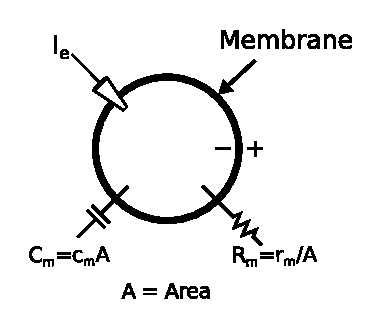
\includegraphics[width=0.45\textwidth]{iso_electrical_model}
    \caption{Diagram of the isopotential neuron. Adapted from Theoretical Neuroscience by Dayan and Abbott~\cite{dayan2001theoretical}.}
  \end{center}
\end{figure}


\subsubsection{Integrate and fire}
This is one of the oldest neuron models, but it's still being used
\subsubsection{Hodgkin-Huxley}

\subsubsection{Leaky integrate and fire}

\subsubsection{Simple model}
izhikevich